\documentclass[book.tex]{subfiles}
\begin{document}
\section{Programming}
\label{section:programming}



Development was done with Borland C++ 3.1 (but the language used was C) which by default ran in EGA mode 3 offering a screen 80 characters wide and 25 characters tall.\\
\par
John Carmack took care of the runtime code. John Romero programmed many of the tools (TED5 map editor, IGRAB asset packer, MUSE sound packer). Jason Blochowiak wrote important subsystems of the game (Input manager, Sound manager, User manager).\\
\par
Borland's solution was an all-in-one package. The IDE, \cw{BC.EXE}, despite some instabilities allowed crude multi-windows code editing with pleasant syntax highlights. The compiler and linker were also part of the package under \cw{BCC.EXE} and \cw{TLINK.EXE}\footnote{Source: Borland C++ 3.1 User Guide.}.\\

\begin{figure}[H]
\centering
  \fullimage{compiling.png}
\caption{Borland C++ 3.1 editor}
\end{figure}
\par

\pagebreak


There was no need to enter command-line mode however. The IDE allowed to create a project, build, run and debug.\\
\par
\begin{figure}[H]
\centering
  \fullimage{borland_compile.png}
  \caption{Compiling Keen Dreams with Borland C++ 3.1}
\end{figure}






Another way to improve screen real estate was to use "high resolution" 50x80 text mode.\\
\par 
 \fullimage{borland_ide_select.png}\\
 \par
 \vspace{-7pt}
The comments still fit perfectly on screen since only the vertical resolution is doubled.\\
\par
\vspace{-4pt}
 \fullimage{borland_ide_highres.png}
 
\bigskip
 The file \cw{KD\_MAIN.C} opened in both modes demonstrates the readability/visibility trade-off.\\
\par

  \fullimage{borland_ide_main_lowres.png}\\
\vspace{-5pt}  
   %\vspace{-4pt}
\par
\vspace{5pt}
 \fullimage{borland_ide_main_highres.png}
\section{Graphic Assets}
\label{section:graphic_assets}

All graphic assets were produced by Adrian Carmack. All of the work was done with Deluxe Paint (by Brent Iverson, Electronic Arts) and saved in ILBM\footnote{InterLeaved BitMap.} files (Deluxe Paint proprietary format). All assets were hand drawn with a mouse.

\begin{figure}[H]
  \centering
 \fullimage{deluxe_paint.png}
 \caption{Deluxe Paint was used to draw all assets in the game.}
\end{figure}

\pagebreak

\subsection{Assets Workflow}
After the graphic assets were generated, a tool (IGRAB) packed all ILBMs together in a compressed \cw{DATA} archive (\cw{EGA}-file) and generated a \cw{HEAD} table, \cw{DICT} file (\cw{KDR}-files\footnote{both \cw{KDR}-files are located in the \cw{static} folder of the source code.}) and C header file with asset IDs. The engine references an asset directly by using these IDs.\\

\begin{figure}[H]
\centering
 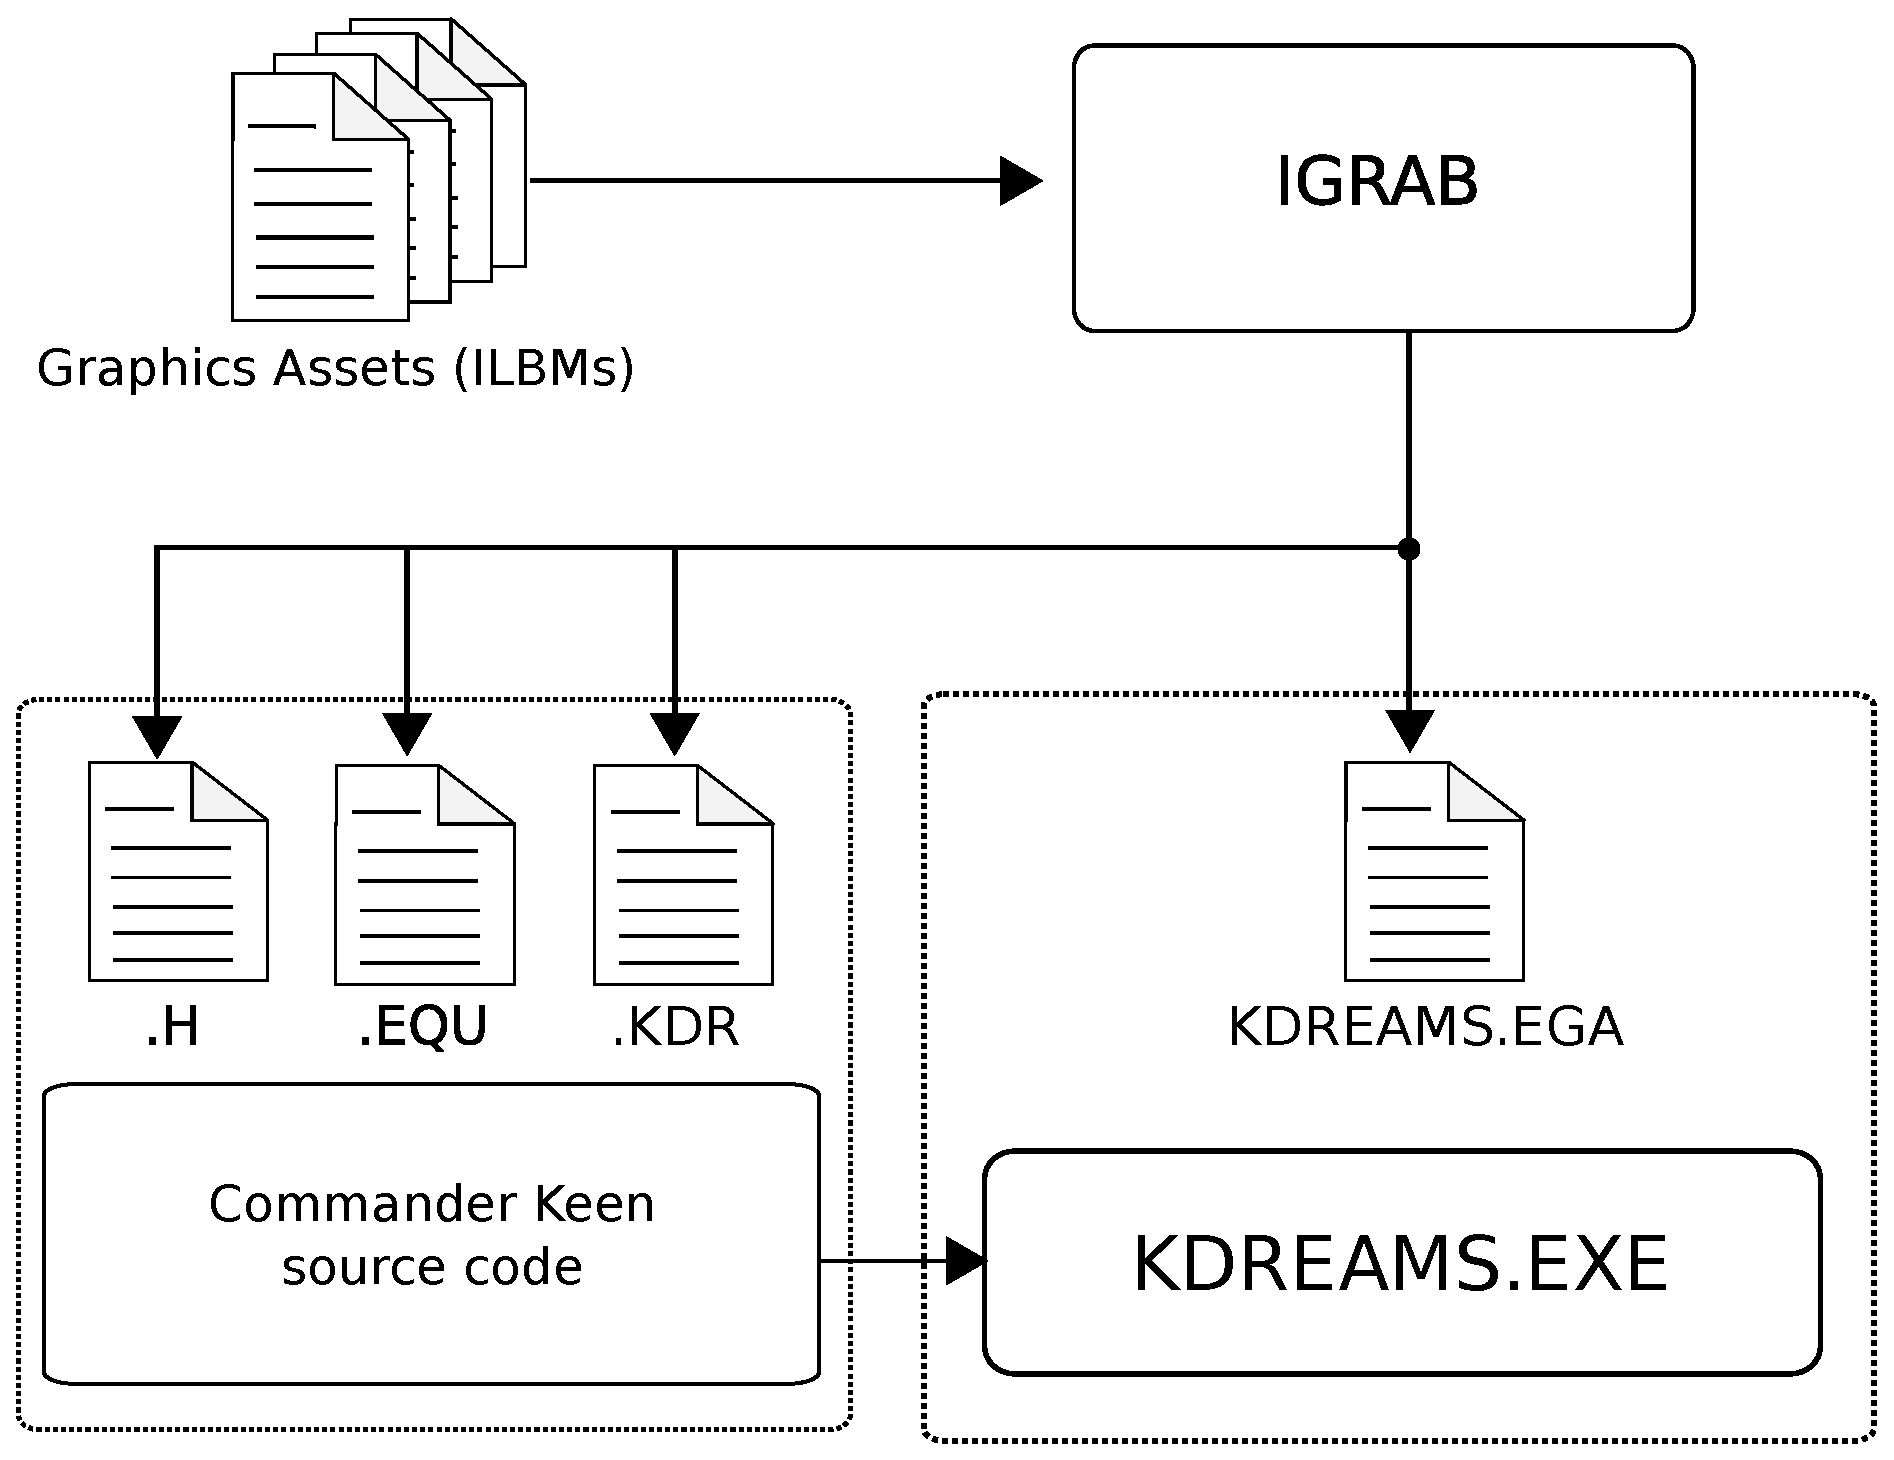
\includegraphics[width=.9\textwidth]{imgs/drawings/drawing_plain.eps}
 \caption{Asset creation pipeline for graphics items}
 \label{asset-creation-pipeline}
\end{figure}

\par
In the engine code, asset usage is hardcoded via an enum. This enum is an offset into
the \cw{HEAD} table which gives an offset in the \cw{DATA} archive. With this indirection layer, assets could be regenerated and reordered at will with no modification in the source code. \\

\trivia{The \cw{HEAD} and \cw{DICT} files in the source code must match the \cw{DATA} file from the shareware version of Keen Dreams. The latest release of the source code (v1.93) doesn't match with the final shareware version 1.13. You need to retrieve a specific \cw{git} commit to ensure a \cw{HEAD}, \cw{DICT} and \cw{DATA} archive are matching, which will be explained in the next chapter.}

\par
\begin{minipage}{\textwidth}
 \lstinputlisting[language=C]{code/assets_header.c}\par
 \end{minipage}
 


 

\subsection{Assets archive file structure}
\label{section:asset_file_structure}
Figure \ref{fig:asset-file} shows the structure of the \cw{KDREAMS.EGA} asset archive file. The first sections contains data tables for pictures and sprites, followed by the font and all sprites and tiles.\\
\begin{figure}[H]
\centering
 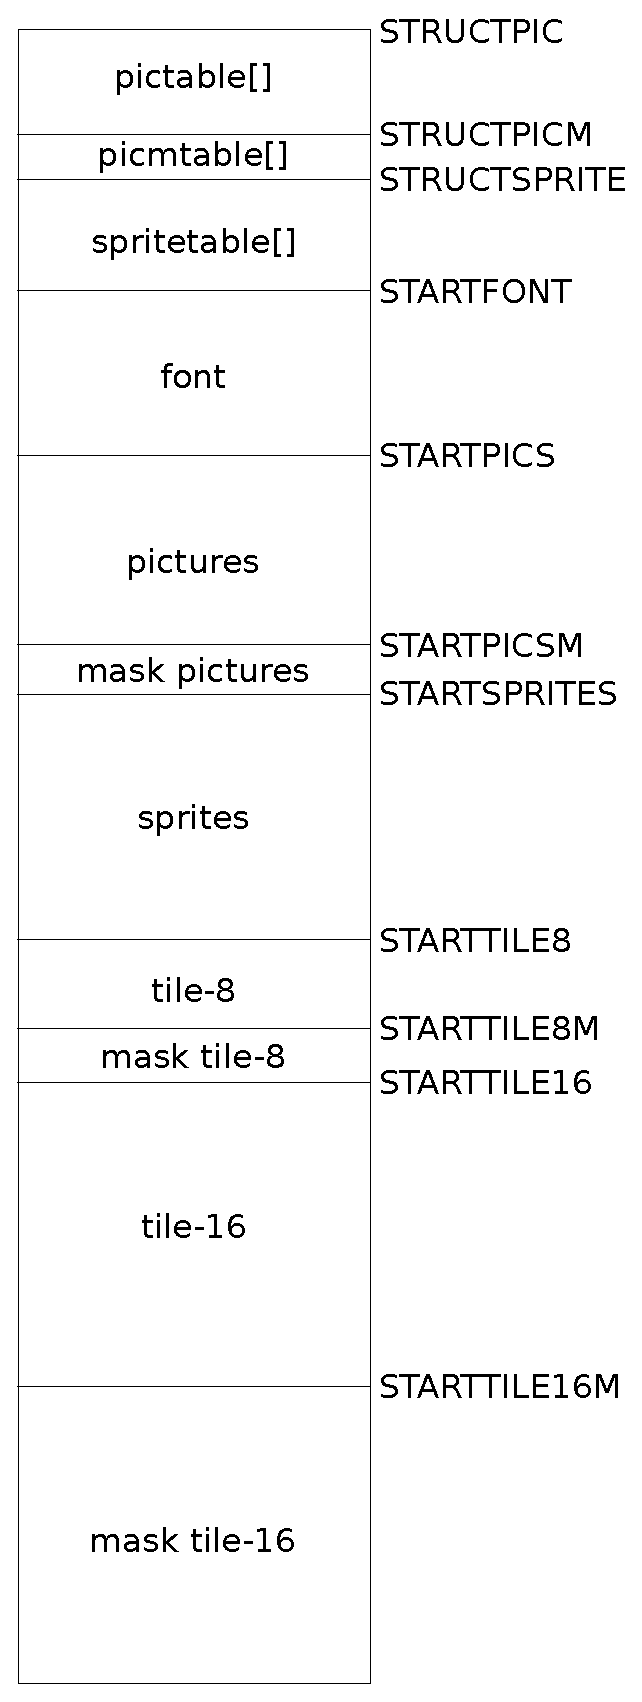
\includegraphics[width=.4\textwidth]{imgs/drawings/graphic_assets.eps}
 \caption{File structure of \cw{KDREAMS.EGA} archive file.}
 \label{fig:asset-file}
\end{figure}

Boh the \textbf{pictable[]} and \textbf{picmtable[]} contain the width and height for each (masked) picture in the asset file.\\

  \begin{table}[H]
  \begin{tabularx}{0.8\textwidth}[c]{XXX}
  \hline
  \textbf{picture index} & \textbf{width (bytes)} & \textbf{height (bytes)}   \\ \hline
  0             & 5          & 32    \\
  1             & 5          & 32    \\
  2             & 5          & 32    \\
  3             & 5          & 32    \\
  4             & 5          & 32    \\
  5             & 5          & 32    \\
  6             & 5          & 32    \\
  7             & 5          & 32    \\
  ...             & ...          & ...    \\
  64             & 5          & 24    \\
  \end{tabularx}
  %\caption{content of \cw{pictable[]} and \cw{picmtable[]}.}
  \end{table}



The \textbf{spritetable[]} contains, beside width and height, also information on the sprite center, hit boundaries and number of bitshifts. Sprites will be explained in detail in section \ref{section:draw_sprites} on page \pageref{section:draw_sprites}. \\

\par
\begin{minipage}{\textwidth}
 \lstinputlisting[language=C]{code/font_structure.c}\par
 \end{minipage}

\par
The \textbf{font} segment contains a table for the height (same for all characters) and width of the font, as well as a reference where the character data is located in the archive file.\\

\begin{figure}[H] 
  \centering 
  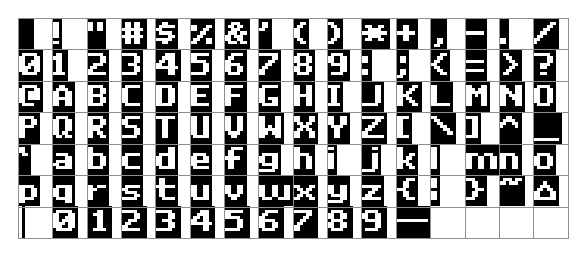
\includegraphics[width=1.0\textwidth]{imgs/drawings/font.eps}
  \caption{Font asset data.}
  \label{fig:font_assets}
\end{figure} 

\par
The remainder of the archive file contains all graphic assets, including pictures, sprites and tiles. Each asset contains four planes, aligned with the EGA architecture. All masked tiles and sprites include an additional mask plane as well.
 
\begin{figure}[H]
\centering
 \begin{table}[H]
  \begin{tabularx}{\textwidth}[c]{XXXXXX}
  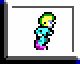
\includegraphics[width=0.15\textwidth]{screenshots_300dpi/game/picture1.png} &
  
\includegraphics[width=0.15\textwidth]{screenshots_300dpi/game/picture2.png} &
  
\includegraphics[width=0.15\textwidth]{screenshots_300dpi/game/picture3.png} &
  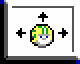
\includegraphics[width=0.15\textwidth]{screenshots_300dpi/game/picture4.png} &
  
\includegraphics[width=0.15\textwidth]{screenshots_300dpi/game/picture5.png} &
  
\includegraphics[width=0.15\textwidth]{screenshots_300dpi/game/picture6.png} \\
  
\includegraphics[width=0.15\textwidth]{screenshots_300dpi/game/picture7.png} &
  
\includegraphics[width=0.15\textwidth]{screenshots_300dpi/game/picture8.png} &
  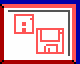
\includegraphics[width=0.15\textwidth]{screenshots_300dpi/game/picture9.png} &
  
\includegraphics[width=0.15\textwidth]{screenshots_300dpi/game/picture10.png} &
  
\includegraphics[width=0.15\textwidth]{screenshots_300dpi/game/picture11.png} &
  
\includegraphics[width=0.15\textwidth]{screenshots_300dpi/game/picture12.png} \\
  
\includegraphics[width=0.15\textwidth]{screenshots_300dpi/game/picture13.png} &
  
\includegraphics[width=0.15\textwidth]{screenshots_300dpi/game/picture14.png} &
  
\includegraphics[width=0.15\textwidth]{screenshots_300dpi/game/picture15.png} &
  
\includegraphics[width=0.15\textwidth]{screenshots_300dpi/game/picture16.png} &
  
\includegraphics[width=0.15\textwidth]{screenshots_300dpi/game/picture17.png} &
  
\includegraphics[width=0.15\textwidth]{screenshots_300dpi/game/picture18.png} \\
  
\includegraphics[width=0.15\textwidth]{screenshots_300dpi/game/picture19.png} &
  
\includegraphics[width=0.15\textwidth]{screenshots_300dpi/game/picture20.png} &
  
\includegraphics[width=0.15\textwidth]{screenshots_300dpi/game/picture21.png} &
  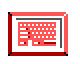
\includegraphics[width=0.15\textwidth]{screenshots_300dpi/game/picture22.png} &
  
\includegraphics[width=0.15\textwidth]{screenshots_300dpi/game/picture23.png} &
  
\includegraphics[width=0.15\textwidth]{screenshots_300dpi/game/picture24.png} \\
  \end{tabularx}
  \end{table}
  \caption{Picture assets.}
  \label{fig:picture_assets}
 \end{figure} 
 

\begin{figure}[H]
\centering
 \begin{table}[H]
  \begin{tabularx}{\textwidth}[c]{|XXXXXX|}
  \hline
  
\includegraphics[width=0.18\textwidth]{screenshots_300dpi/game/sprite1a.png} &
  
\includegraphics[width=0.18\textwidth]{screenshots_300dpi/game/sprite1b.png} &
  
\includegraphics[width=0.18\textwidth]{screenshots_300dpi/game/sprite1c.png} &
  
\includegraphics[width=0.18\textwidth]{screenshots_300dpi/game/sprite1d.png} &
  
\includegraphics[width=0.18\textwidth]{screenshots_300dpi/game/sprite1e.png} &
  
\includegraphics[width=0.18\textwidth]{screenshots_300dpi/game/sprite1f.png} \\  
  
\includegraphics[width=0.18\textwidth]{screenshots_300dpi/game/sprite1g.png} & 
  
\includegraphics[width=0.18\textwidth]{screenshots_300dpi/game/sprite1h.png} &
  
\includegraphics[width=0.18\textwidth]{screenshots_300dpi/game/sprite2a.png} &
  
\includegraphics[width=0.18\textwidth]{screenshots_300dpi/game/sprite2b.png} &
  
\includegraphics[width=0.18\textwidth]{screenshots_300dpi/game/sprite2c.png} &
  
\includegraphics[width=0.18\textwidth]{screenshots_300dpi/game/sprite2d.png} \\  
  
\includegraphics[width=0.18\textwidth]{screenshots_300dpi/game/sprite2e.png} &
  
\includegraphics[width=0.18\textwidth]{screenshots_300dpi/game/sprite2f.png} &
  
\includegraphics[width=0.18\textwidth]{screenshots_300dpi/game/sprite2g.png} & 
  
\includegraphics[width=0.18\textwidth]{screenshots_300dpi/game/sprite2h.png} & & \\  
  \multicolumn{6}{|c|}{BROCCOLASH}  \\ \hline
  \multicolumn{6}{c}{}  \\ \hline
    
  
\includegraphics[width=0.18\textwidth]{screenshots_300dpi/game/sprite3a.png} &
  
\includegraphics[width=0.18\textwidth]{screenshots_300dpi/game/sprite3b.png} &  
  
\includegraphics[width=0.18\textwidth]{screenshots_300dpi/game/sprite3c.png} &
  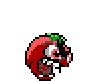
\includegraphics[width=0.18\textwidth]{screenshots_300dpi/game/sprite3d.png} & & \\  
  \multicolumn{6}{|c|}{TOMATOOTH}  \\ \hline
  \multicolumn{6}{c}{}  \\ \hline      
  
  
\includegraphics[width=0.18\textwidth]{screenshots_300dpi/game/sprite3e.png} &
  
\includegraphics[width=0.18\textwidth]{screenshots_300dpi/game/sprite3f.png} &
  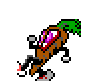
\includegraphics[width=0.18\textwidth]{screenshots_300dpi/game/sprite3g.png} & 
  \includegraphics[width=0.18\textwidth]{screenshots_300dpi/game/sprite3h.png} &   
  \includegraphics[width=0.18\textwidth]{screenshots_300dpi/game/sprite4a.png} &
  \includegraphics[width=0.18\textwidth]{screenshots_300dpi/game/sprite4b.png} \\    
  \includegraphics[width=0.18\textwidth]{screenshots_300dpi/game/sprite4c.png} &
  \includegraphics[width=0.18\textwidth]{screenshots_300dpi/game/sprite4d.png} &
  \includegraphics[width=0.18\textwidth]{screenshots_300dpi/game/sprite4e.png} & 
  \includegraphics[width=0.18\textwidth]{screenshots_300dpi/game/sprite4f.png} & & \\
  \multicolumn{6}{|c|}{CARROT}  \\ \hline
  \multicolumn{6}{c}{}     
  \end{tabularx}
  \end{table}
  \caption{Sprite assets.}
  \label{fig:sprite_assets}
 \end{figure}


\pagebreak
\begin{figure}[H] 
  \centering 
  \includegraphics[width=0.99\textwidth, frame]{screenshots_300dpi/tile16_assets.png}
\end{figure}  

\begin{figure}[H] 
  \centering 
  \includegraphics[width=0.99\textwidth, frame]{screenshots_300dpi/tile16M_assets.png}
  \caption{Background (Tile-16) and foreground (masked Tile-16) assets.}
  \label{fig:tile16_assets}
\end{figure} 



\section{Maps}
Maps were created using an in-house editor called TED5, short for Tile EDitor. Over the years TED5 had improvements and the same tool is later used for creating maps for both side-scrolling games and top-down games like \textit{Wolfenstein 3D}.\\
\par
 TED5 is not stand-alone; in order to start, it needs an asset archive and the  associated header (as described in the graphic asset workflow Figure \ref{asset-creation-pipeline} on page \pageref{asset-creation-pipeline}). This way, tile IDs are directly encoded in the map.\\

 
 \fullimage{TedSplashscreen.png}
 \par
 \trivia{The suffix, "vD.IP", was put in by the Rise of the Triad team in 1994. It stood for "Developers of Incredible Power".}\\
 \par
\fullimage{Fill_2.png}\\
 
 \par
TED5 allows placement of tiles on layers called "planes". In Commander Keen, there are three type of planes:
\begin{itemize}
  \item Background plane tiles
  \item Foreground plane tiles, which is a mask over the background plane
  \item Information plane tiles, containing location of actors and special places
\end{itemize}
A level is created by placing tiles on each of these three layers. Each foreground and background tile could be enriched with additional tile information. It controls how everything interacts with tiles, like tile clipping, "deadly" tiles and animated tiles. \\

 \par
\fullimage{ted5_tile_info.png}\\
 
 \par

Just like IGRAB, the TED5 tool packed all levels together in a compressed \cw{MAP} archive and generated a \cw{HEAD} and \cw{DICT} file (\cw{KDR}-extension). \\
 
\subsection{Map header structure}
The map header structure is part of the engine code and contains a header offset and size, which refers to the location and size in the \cw{KDREAMS.MAP} archive file. \\

\par
\begin{minipage}{\textwidth}
 \lstinputlisting[language=C]{code/map_header_structure.c}\par
 \end{minipage}

A maximum of 100 maps is supported in the game. The \cw{tileinfo[]} data contains information for tile interaction. 


 
\begin{figure}[H]
\centering
 \includegraphics[width=1.0\textwidth]{imgs/drawings/map_header.eps}
 \caption{Structure of \cw{MAPHEAD.KDR} header file.}
 \label{fig:map-header-file}
\end{figure}
\par

For background tile animation two information tables are defined: \textbf{tile animation} and \textbf{tile animation speed}. The tile animation refers which tile, relative to this tile, the tile will animate to. In Table \ref{table:background tile anim} the next animation after tile \#90 is \#91 (+1), followed by \#92 (+1) and \#93 (+1). After tile \#93 (-3) the sequence is going back to tile \#90. The animation speed is expressed in number of ticks before the next tile is displayed. \\
 \begin{table}[H]
  \begin{tabularx}{\textwidth}[c]{XXX}
  \hline
  \textbf{index} & \textbf{tile animation} & \textbf{tile animation speed}   \\ \hline
  0             & 0          & 0    \\
  1             & 0          & 0    \\
  ...             & ...          & ...    \\
  57             & 1          & 32    \\
  58             & -1          & 24    \\
  ...             & ...          & ...    \\
  90             & 1          & 8    \\
  91            & 1          & 8    \\
  92             & 1          & 8    \\
  93             & -3          & 8    \\
  ...             & ...          & ...    \\
  \end{tabularx}
  \caption{Background tile animation.}
  \label{table:background tile anim}
  \end{table}
  
  \par
The foreground tiles contain, beside tile animation (similar like background tiles), also clipping and 'inside' tile information.\\
\par
The clipping tables contain how Commander Keen is clipped against foreground tiles. 'Inside' tile information is used to climb on a pole and mimics Commander Keen going through a floor opening ('inside' the tile). In section \ref{section:clipping} (see page \pageref{section:clipping}) both the clipping and 'inside' logic is further explained.\\
\begin{table}[H]
  \begin{tabularx}{\textwidth}[c]{XXXXXXX}
  \hline
  \textbf{index} & \textbf{clip north} & \textbf{clip east} & \textbf{clip south} & \textbf{clip west}  & \textbf{inside tile} \\ \hline
  ...    & ...     & ...    & ...   & ...     & ...      \\
  238    & 0       & 1      & 5     & 0       & 0        \\
  239    & 0       & 0      & 0     & 0       & 0        \\
  240    & 0       & 0      & 5     & 0       & 0        \\
  241    & 0       & 0      & 0     & 0       & 128       \\
  242    & 1       & 1      & 1     & 1       & 128       \\
  243    & 1       & 0      & 1     & 0       & 0       \\
  244    & 0       & 0      & 2     & 0       & 0       \\
  ...    & ...     & ...    & ...   & ...     & ...     \\
  \end{tabularx}
  \caption{Foreground tile clipping and 'inside' tile information.}
  \end{table}


\pagebreak
 
\subsection{Map archive structure}
The structure of \cw{KDREAMS.MAP} archive is explained in Figure \ref{fig:map-file}. For each map there is a small header containing the width, height and name of the map as well as a reference pointer to each of the three planes. Each plane exists out of a map of tile numbers for background, foreground and info.\\



\par
\begin{minipage}{\textwidth}
 \lstinputlisting[language=C]{code/map_header.c}\par
 \end{minipage}
 
\par
\begin{figure}[H]
\centering
 \includegraphics[width=0.85\textwidth]{imgs/drawings/kdreams_map.eps}
 \caption{Structure of \cw{KDREAMS.MAP} file.}
 \label{fig:map-file}
\end{figure}

\section{Audio}
\subsection{Sounds}
The original Commander Keen Trilogy did only support the default PC Speaker. With the introduction of Commander Keen in Keen Dreams the team decided to support sound cards as well.\\

\par
\bu{Trivia :} Apogee, the publisher of Ideas from the Deep, didn't publish any game with AdLib support until \textit{Dark Ages} in 1991. And even then it still had pc speaker music.\\
\par

id Software intended for Keen Dreams to have music and digital effects support for the SoundBlaster \& Sound Source devices. In fact, Bobby Prince composed the song "You've Got to Eat Your Vegetables!!" for the game's introduction. However, Softdisk Publishing wanted Keen Dreams to fit on a single 360K floppy disk, and in order to do this, id Software had to scrap the game's music at the last minute. The team didn't even have time to remove the music setup menu.\\

\par
\par
\begin{figure}[H]
\centering
\scaledimage{1.0}{music.png}{}
\caption{Setup music menu in Keen Dreams, although there is no music in the game.}
\end{figure}
\par

\pagebreak

\bu{Trivia :} The song "You've Got to Eat Your Vegetables!!" would finally make its debut in Commander Keen IV: Secret of the Oracle.\\
\par

As a consequence, only two sets of each audio effect are shipped with the game:
\begin{enumerate}
\item For PC Speaker
\item For AdLib
\end{enumerate}

Game music was not introduced until Commander Keen IV.  \\

\par
All sound effects are done by Robert Prince. Sound effects are created using Cakewalk and inhouse MUSE tool, which is  extensively described in \textit{Wolfenstein 3D}\footnote{See Wolfenstein 3D Blackbook, section 3.6 on page 94.}
Just like described before, the MUSE tool packed all sound effects together in a compressed \cw{SOUND} archive and generated a \cw{HEAD}, \cw{DICT} file and a C header file with asset IDs.\\




\section{Distribution}
On December 14th, 1990 the first episode was released via Apogee. Episodes 1-5 are all published by Apogee Software. The game engine and first episode were given for free and encourages to be copied and distributed to a maximum number of people. To receive the other episodes, each player had to pay \$30 (for Episode 1-3) to \textit{ideas from the Deep}.\\

\par
Commander Keen in Keen Dreams was published as a retail title by Softdisk, as part of a settlement for using Softdisk resources to make their own game\footnote{The settlement with Softdisk is explained in Appendix \ref{sec:id_software}}.\\

\par
\begin{figure}[H]
\centering
\scaledimage{0.7}{shareware.jpg}{}
\caption{Retail version of Commander Keen in Keen Dreams by Softdisk.}
\end{figure}
\par


In 1990, the Internet was still in its infancy and the best medium was the 3\nicefrac{1}{2}-inch floppy disk. The game shipped as follows:\\

  \par
 The files can be divided in seven parts:
\begin{itemize}
 \item KDREAMS.EXE: Game engine.
 \item KDREAMS.EGA: Contains all the assets (sprites, tiles) needed during the game.
 \item KDREAMS.AUD: Sound effect files.
 \item KDREAMS.MAP: Contains all levels layouts.
 \item KDREAMS.CMP: Introduction picture of the game, which is a compressed LBM image file.
 \item Softdisk Help Library files, which are text screens, shown when starting the game
 \begin{itemize}
   \item START.EXE: Decompress and show user guide, and then start the game.
   \item LOADSCN.EXE: Shows the closing screen when quitting the game. Decompresses the ENDSCN.SCN chunk in LAST.SHL
   \item *.SHL: Text user guide assets. 
 \end{itemize}
 \item Several *.TXT files which can be read in DOS by typing the corresponding *.BAT file. 

\end{itemize}

\par
 \begin{figure}[H]
\centering
 \fullimage{dos_result.png}
 \caption{All Keen Dreams files as they appear in DOS command prompt.}
  \end{figure}
 \par


\end{document}
